\documentclass{report}\usepackage[]{graphicx}\usepackage[]{color}
%% maxwidth is the original width if it is less than linewidth
%% otherwise use linewidth (to make sure the graphics do not exceed the margin)
\makeatletter
\def\maxwidth{ %
  \ifdim\Gin@nat@width>\linewidth
    \linewidth
  \else
    \Gin@nat@width
  \fi
}
\makeatother

\definecolor{fgcolor}{rgb}{0.345, 0.345, 0.345}
\newcommand{\hlnum}[1]{\textcolor[rgb]{0.686,0.059,0.569}{#1}}%
\newcommand{\hlstr}[1]{\textcolor[rgb]{0.192,0.494,0.8}{#1}}%
\newcommand{\hlcom}[1]{\textcolor[rgb]{0.678,0.584,0.686}{\textit{#1}}}%
\newcommand{\hlopt}[1]{\textcolor[rgb]{0,0,0}{#1}}%
\newcommand{\hlstd}[1]{\textcolor[rgb]{0.345,0.345,0.345}{#1}}%
\newcommand{\hlkwa}[1]{\textcolor[rgb]{0.161,0.373,0.58}{\textbf{#1}}}%
\newcommand{\hlkwb}[1]{\textcolor[rgb]{0.69,0.353,0.396}{#1}}%
\newcommand{\hlkwc}[1]{\textcolor[rgb]{0.333,0.667,0.333}{#1}}%
\newcommand{\hlkwd}[1]{\textcolor[rgb]{0.737,0.353,0.396}{\textbf{#1}}}%

\usepackage{framed}
\makeatletter
\newenvironment{kframe}{%
 \def\at@end@of@kframe{}%
 \ifinner\ifhmode%
  \def\at@end@of@kframe{\end{minipage}}%
  \begin{minipage}{\columnwidth}%
 \fi\fi%
 \def\FrameCommand##1{\hskip\@totalleftmargin \hskip-\fboxsep
 \colorbox{shadecolor}{##1}\hskip-\fboxsep
     % There is no \\@totalrightmargin, so:
     \hskip-\linewidth \hskip-\@totalleftmargin \hskip\columnwidth}%
 \MakeFramed {\advance\hsize-\width
   \@totalleftmargin\z@ \linewidth\hsize
   \@setminipage}}%
 {\par\unskip\endMakeFramed%
 \at@end@of@kframe}
\makeatother

\definecolor{shadecolor}{rgb}{.97, .97, .97}
\definecolor{messagecolor}{rgb}{0, 0, 0}
\definecolor{warningcolor}{rgb}{1, 0, 1}
\definecolor{errorcolor}{rgb}{1, 0, 0}
\newenvironment{knitrout}{}{} % an empty environment to be redefined in TeX

\usepackage{alltt}

\title{Thesis 2014 - Figures}
\IfFileExists{upquote.sty}{\usepackage{upquote}}{}

\begin{document}
\maketitle


This is the file I used for all animated figures used in my thesis defence.
\begin{knitrout}
\definecolor{shadecolor}{rgb}{0.969, 0.969, 0.969}\color{fgcolor}\begin{kframe}
\begin{alltt}
\hlkwd{cat}\hlstd{(}\hlstr{"Hello World\textbackslash{}n"}\hlstd{)}
\end{alltt}
\begin{verbatim}
## Hello World
\end{verbatim}
\end{kframe}
\end{knitrout}


Try to animation package. I think I will be using ImageMagick and SWFtools.
\begin{knitrout}
\definecolor{shadecolor}{rgb}{0.969, 0.969, 0.969}\color{fgcolor}\begin{kframe}
\begin{alltt}
\hlkwd{require}\hlstd{(animation)}
\end{alltt}
\end{kframe}
\end{knitrout}


Simulate static data.
\begin{knitrout}
\definecolor{shadecolor}{rgb}{0.969, 0.969, 0.969}\color{fgcolor}\begin{kframe}
\begin{alltt}
\hlstd{x} \hlkwb{<-} \hlkwd{rnorm}\hlstd{(}\hlnum{100}\hlstd{)}
\hlstd{y} \hlkwb{<-} \hlnum{5} \hlopt{+} \hlnum{2} \hlopt{*} \hlstd{x} \hlopt{-} \hlnum{4} \hlopt{*} \hlstd{x}\hlopt{^}\hlnum{2}
\hlstd{fit} \hlkwb{<-} \hlkwd{lm}\hlstd{(y} \hlopt{~} \hlstd{x)}
\hlkwd{plot}\hlstd{(y} \hlopt{~} \hlstd{x,} \hlkwc{col} \hlstd{=} \hlstr{"chocolate"}\hlstd{,} \hlkwc{pch} \hlstd{=} \hlnum{20}\hlstd{)}
\hlkwd{abline}\hlstd{(fit,} \hlkwc{col} \hlstd{=} \hlstr{"forestgreen"}\hlstd{,} \hlkwc{lwd} \hlstd{=} \hlnum{2}\hlstd{)}
\hlstd{pred} \hlkwb{<-} \hlkwd{predict}\hlstd{(fit)}
\hlkwd{segments}\hlstd{(x, y, x, pred,} \hlkwc{lty} \hlstd{=} \hlstr{"dashed"}\hlstd{)}
\hlkwd{points}\hlstd{(x, pred,} \hlkwc{pch} \hlstd{=} \hlnum{4}\hlstd{,} \hlkwc{cex} \hlstd{=} \hlnum{0.5}\hlstd{)}
\end{alltt}
\end{kframe}
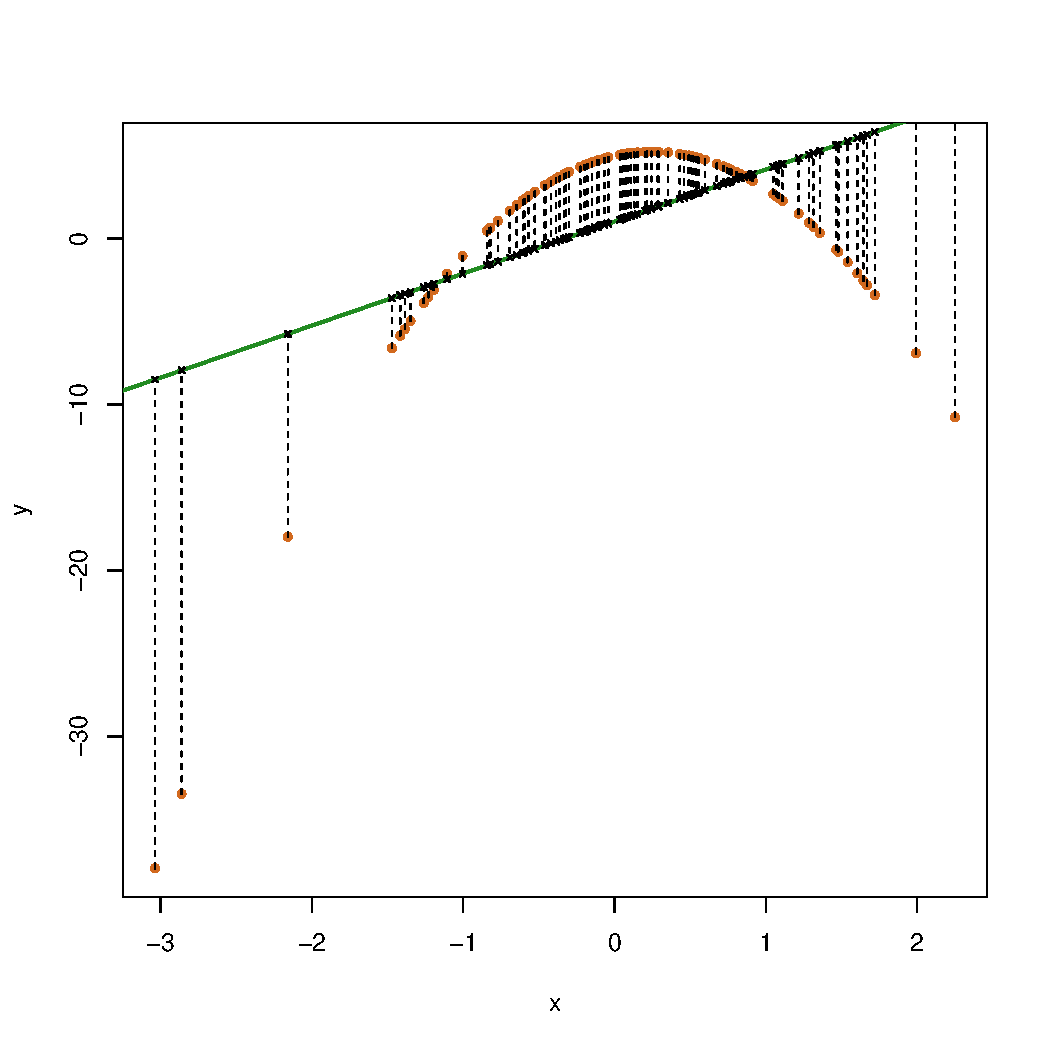
\includegraphics[width=\maxwidth]{figure/unnamed-chunk-3} 

\end{knitrout}


Build a function to draw a \textbf{static} simulated data.
\begin{knitrout}
\definecolor{shadecolor}{rgb}{0.969, 0.969, 0.969}\color{fgcolor}\begin{kframe}
\begin{alltt}
\hlstd{lineaire} \hlkwb{<-} \hlkwa{function}\hlstd{(}\hlkwc{a}\hlstd{) \{}
    \hlstd{x} \hlkwb{<-} \hlkwd{rnorm}\hlstd{(a)}
    \hlstd{y} \hlkwb{<-} \hlnum{10} \hlopt{*} \hlstd{x} \hlopt{-} \hlstd{x}\hlopt{^}\hlnum{3}
    \hlstd{fit} \hlkwb{<-} \hlkwd{lm}\hlstd{(y} \hlopt{~} \hlstd{x)}
    \hlkwd{plot}\hlstd{(y} \hlopt{~} \hlstd{x,} \hlkwc{col} \hlstd{=} \hlstr{"chocolate"}\hlstd{,} \hlkwc{pch} \hlstd{=} \hlnum{20}\hlstd{)}
    \hlkwd{abline}\hlstd{(fit,} \hlkwc{col} \hlstd{=} \hlstr{"forestgreen"}\hlstd{,} \hlkwc{lwd} \hlstd{=} \hlnum{2}\hlstd{)}
\hlstd{\}}
\hlkwd{lineaire}\hlstd{(}\hlnum{100}\hlstd{)}
\end{alltt}
\end{kframe}
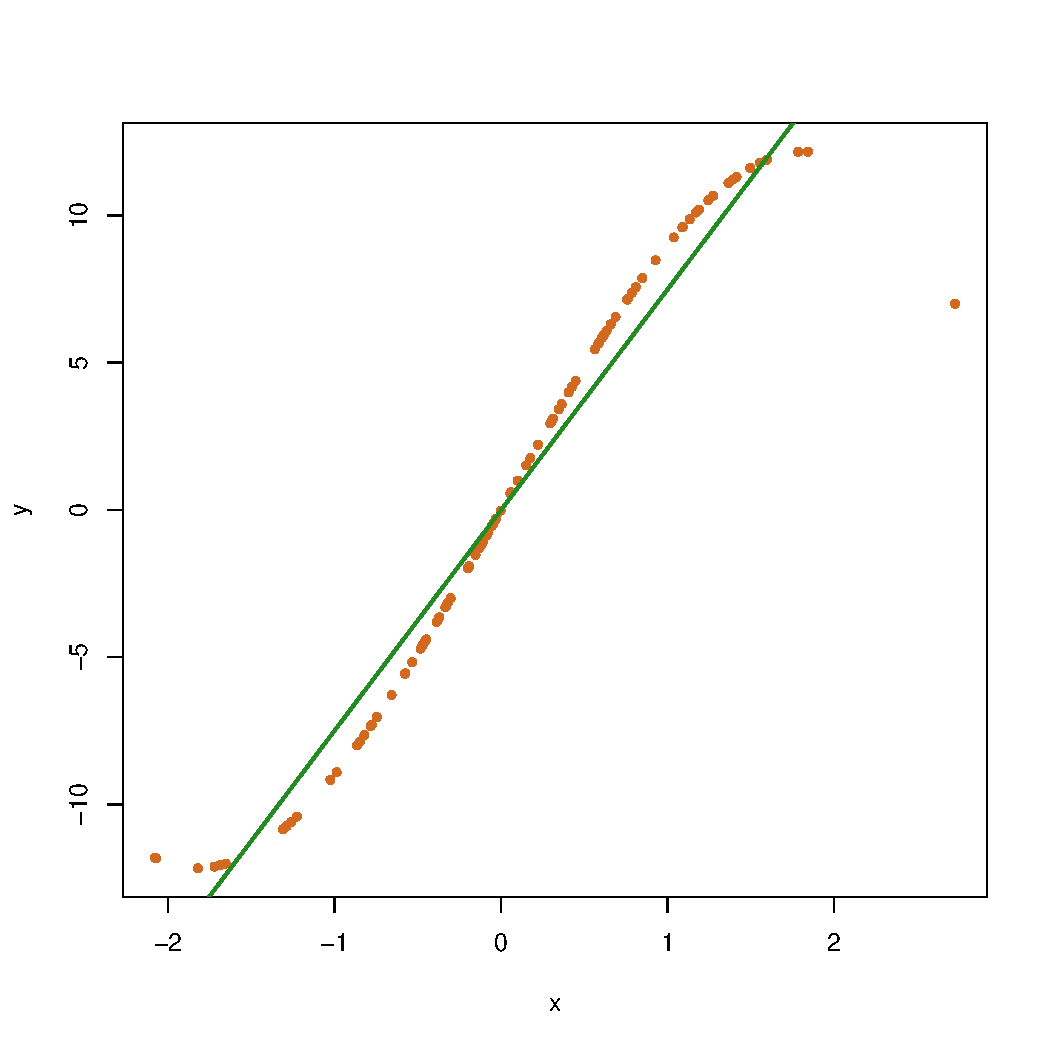
\includegraphics[width=\maxwidth]{figure/unnamed-chunk-4} 

\end{knitrout}



Try to animate a for loop.
\begin{knitrout}
\definecolor{shadecolor}{rgb}{0.969, 0.969, 0.969}\color{fgcolor}\begin{kframe}
\begin{alltt}
\hlstd{frames} \hlkwb{=} \hlnum{100}

\hlkwa{for} \hlstd{(i} \hlkwa{in} \hlnum{1}\hlopt{:}\hlstd{frames) \{}
    \hlcom{## create a name for each plot}
    \hlkwa{if} \hlstd{(i} \hlopt{<} \hlnum{10}\hlstd{) \{}
        \hlstd{name} \hlkwb{=} \hlkwd{paste}\hlstd{(}\hlstr{"000"}\hlstd{, i,} \hlstr{"plot.png"}\hlstd{,} \hlkwc{sep} \hlstd{=} \hlstr{""}\hlstd{)}
    \hlstd{\}}
    \hlkwa{if} \hlstd{(i} \hlopt{<} \hlnum{100} \hlopt{&&} \hlstd{i} \hlopt{>=} \hlnum{10}\hlstd{) \{}
        \hlstd{name} \hlkwb{=} \hlkwd{paste}\hlstd{(}\hlstr{"00"}\hlstd{, i,} \hlstr{"plot.png"}\hlstd{,} \hlkwc{sep} \hlstd{=} \hlstr{""}\hlstd{)}
    \hlstd{\}}
    \hlkwa{if} \hlstd{(i} \hlopt{>=} \hlnum{100}\hlstd{) \{}
        \hlstd{name} \hlkwb{=} \hlkwd{paste}\hlstd{(}\hlstr{"0"}\hlstd{, i,} \hlstr{"plot.png"}\hlstd{,} \hlkwc{sep} \hlstd{=} \hlstr{""}\hlstd{)}
    \hlstd{\}}

    \hlstd{x} \hlkwb{<-} \hlkwd{rnorm}\hlstd{(frames)}
    \hlstd{y} \hlkwb{<-} \hlnum{10} \hlopt{*} \hlstd{x[i]} \hlopt{-} \hlstd{x[i]}\hlopt{^}\hlnum{3}
    \hlcom{# fit <- lm(y~x)}

    \hlkwd{png}\hlstd{(name)}
    \hlkwd{plot}\hlstd{(y} \hlopt{~} \hlstd{x,} \hlkwc{pch} \hlstd{=} \hlnum{20}\hlstd{,} \hlkwc{col} \hlstd{=} \hlstr{"chocolate"}\hlstd{)}
    \hlcom{# dev.off()}
\hlstd{\}}
\end{alltt}


{\ttfamily\noindent\bfseries\color{errorcolor}{\#\# Error: variable lengths differ (found for 'x')}}\end{kframe}
\end{knitrout}



Plot the number of species that have been extinct in the wild since 1500.
\begin{knitrout}
\definecolor{shadecolor}{rgb}{0.969, 0.969, 0.969}\color{fgcolor}\begin{kframe}
\begin{alltt}
\hlstd{species} \hlkwb{<-} \hlkwd{read.table}\hlstd{(}\hlstr{"clipboard"}\hlstd{,} \hlkwc{sep} \hlstd{=} \hlstr{"\textbackslash{}t"}\hlstd{,} \hlkwc{header} \hlstd{= T)}
\hlkwd{require}\hlstd{(ggplot2)}
\hlkwd{ggplot}\hlstd{(species,} \hlkwd{aes}\hlstd{(}\hlkwc{x} \hlstd{= Esp�ce,} \hlkwc{y} \hlstd{= Organisme))} \hlopt{+} \hlkwd{geom_bar}\hlstd{(}\hlkwc{colour} \hlstd{=} \hlstr{"black"}\hlstd{,}
    \hlkwc{fill} \hlstd{=} \hlstr{"#DD8888"}\hlstd{,} \hlkwc{width} \hlstd{=} \hlnum{0.7}\hlstd{,} \hlkwc{stat} \hlstd{=} \hlstr{"identity"}\hlstd{)}
\end{alltt}


{\ttfamily\noindent\bfseries\color{errorcolor}{\#\# Error: object 'Esp�ce' not found}}\end{kframe}
\end{knitrout}



\end{document}








